%%%%%%%%%%%%%%%%%%%%%%%%%%%%%%%%%%%%%%%%%
% Proceedings of the National Academy of Sciences (PNAS)
% LaTeX Template
% Version 1.0 (19/5/13)
%
% This template has been downloaded from:
% http://www.LaTeXTemplates.com
%
% Original author:
% The PNAStwo class was created and is owned by PNAS:
% http://www.pnas.org/site/authors/LaTex.xhtml
% This template has been modified from the blank PNAS template to include
% examples of how to insert content and drastically change commenting. The
% structural integrity is maintained as in the original blank template.
%
% Original header:
%% PNAStmpl.tex
%% Template file to use for PNAS articles prepared in LaTeX
%% Version: Apr 14, 2008
%
%%%%%%%%%%%%%%%%%%%%%%%%%%%%%%%%%%%%%%%%%

%----------------------------------------------------------------------------------------
%	PACKAGES AND OTHER DOCUMENT CONFIGURATIONS
%----------------------------------------------------------------------------------------

%------------------------------------------------
% BASIC CLASS FILE
%------------------------------------------------

%% PNAStwo for two column articles is called by default.
%% Uncomment PNASone for single column articles. One column class
%% and style files are available upon request from pnas@nas.edu.

%\documentclass{pnasone}
\documentclass{pnastwo}

%------------------------------------------------
% POSITION OF TEXT
%------------------------------------------------

%% Changing position of text on physical page:
%% Since not all printers position
%% the printed page in the same place on the physical page,
%% you can change the position yourself here, if you need to:

% \advance\voffset -.5in % Minus dimension will raise the printed page on the 
                         %  physical page; positive dimension will lower it.

%% You may set the dimension to the size that you need.

%------------------------------------------------
% GRAPHICS STYLE FILE
%------------------------------------------------

%% Requires graphics style file (graphicx.sty), used for inserting
%% .eps/image files into LaTeX articles.
%% Note that inclusion of .eps files is for your reference only;
%% when submitting to PNAS please submit figures separately.

%% Type into the square brackets the name of the driver program 
%% that you are using. If you don't know, try dvips, which is the
%% most common PC driver, or textures for the Mac. These are the options:

% [dvips], [xdvi], [dvipdf], [dvipdfm], [dvipdfmx], [pdftex], [dvipsone],
% [dviwindo], [emtex], [dviwin], [pctexps], [pctexwin], [pctexhp], [pctex32],
% [truetex], [tcidvi], [vtex], [oztex], [textures], [xetex]

\usepackage{graphicx}

%------------------------------------------------
% OPTIONAL POSTSCRIPT FONT FILES
%------------------------------------------------

%% PostScript font files: You may need to edit the PNASoneF.sty
%% or PNAStwoF.sty file to make the font names match those on your system. 
%% Alternatively, you can leave the font style file commands commented out
%% and typeset your article using the default Computer Modern 
%% fonts (recommended). If accepted, your article will be typeset
%% at PNAS using PostScript fonts.

% Choose PNASoneF for one column; PNAStwoF for two column:
%\usepackage{PNASoneF}
%\usepackage{PNAStwoF}

%------------------------------------------------
% ADDITIONAL OPTIONAL STYLE FILES
%------------------------------------------------

%% The AMS math files are commonly used to gain access to useful features
%% like extended math fonts and math commands.

\usepackage{amssymb,amsfonts,amsmath}

%------------------------------------------------
% OPTIONAL MACRO FILES
%------------------------------------------------

%% Insert self-defined macros here.
%% \newcommand definitions are recommended; \def definitions are supported

\usepackage{algpseudocode}
\usepackage{algorithm}

%\newcommand{\mfrac}[2]{\frac{\displaystyle #1}{\displaystyle #2}}
%\def\s{\sigma}

%------------------------------------------------
% DO NOT EDIT THIS SECTION
%------------------------------------------------

%% For PNAS Only:
\contributor{Submitted to Proceedings of the National Academy of Sciences of the United States of America}
\url{www.pnas.org/cgi/doi/10.1073/pnas.0709640104}
\copyrightyear{2008}
\issuedate{Issue Date}
\volume{Volume}
\issuenumber{Issue Number}

%----------------------------------------------------------------------------------------

\begin{document}

%----------------------------------------------------------------------------------------
%	TITLE AND AUTHORS
%----------------------------------------------------------------------------------------

\title{Learning molecular fingerprints} % For titles, only capitalize the first letter

%------------------------------------------------

%% Enter authors via the \author command.  
%% Use \affil to define affiliations.
%% (Leave no spaces between author name and \affil command)

%% Note that the \thanks{} command has been disabled in favor of
%% a generic, reserved space for PNAS publication footnotes.

%% \author{<author name>
%% \affil{<number>}{<Institution>}} One number for each institution.
%% The same number should be used for authors that
%% are affiliated with the same institution, after the first time
%% only the number is needed, ie, \affil{number}{text}, \affil{number}{}
%% Then, before last author ...
%% \and
%% \author{<author name>
%% \affil{<number>}{}}

%% For example, assuming Garcia and Sonnery are both affiliated with
%% Universidad de Murcia:
%% \author{Roberta Graff\affil{1}{University of Cambridge, Cambridge,
%% United Kingdom},
%% Javier de Ruiz Garcia\affil{2}{Universidad de Murcia, Bioquimica y Biologia
%% Molecular, Murcia, Spain}, \and Franklin Sonnery\affil{2}{}}

\author{John Smith\affil{1}{University of California},
James Smith\affil{2}{University of Oregon}
\and
Jane Smith\affil{1}{}}

\contributor{Submitted to Proceedings of the National Academy of Sciences
of the United States of America}

%----------------------------------------------------------------------------------------

\maketitle % The \maketitle command is necessary to build the title page

\begin{article}

%----------------------------------------------------------------------------------------
%	ABSTRACT, KEYWORDS AND ABBREVIATIONS
%----------------------------------------------------------------------------------------

\begin{abstract}
Predicting the properties of new compounds requires a representation of molecules that allows generalization.
Currently, such representations are based on hand-coded features such as the Morgan circular fingerprints, which have various limitations.
We introduce a set of fingerprints based on convolutional neural nets which generalize commonly-used fingerprints.
\end{abstract}

%------------------------------------------------

\keywords{Keyword1 | Keyword2 | Keyword3} % When adding keywords, separate each term with a straight line: |

%------------------------------------------------

%% Optional for entering abbreviations, separate the abbreviation from
%% its definition with a comma, separate each pair with a semicolon:
%% for example:
%% \abbreviations{SAM, self-assembled monolayer; OTS,
%% octadecyltrichlorosilane}

% \abbreviations{}
\abbreviations{SAM, self-assembled monolayer; OTS, octadecyltrichlorosilane}

%----------------------------------------------------------------------------------------
%	PUBLICATION CONTENT
%----------------------------------------------------------------------------------------

%% The first letter of the article should be drop cap: \dropcap{} e.g.,
%\dropcap{I}n this article we study the evolution of ''almost-sharp'' fronts

\section{Introduction}

\dropcap{N}am fermentum sapien at enim varius consectetur. Quisque lobortis imperdiet mauris, et accumsan libero vulputate vitae. Integer lacinia purus 


\section{Desirable Properties of Molecular Representations}

\begin{itemize}

\item invariant to global orientation
\item invariant to atom re-labeling
\item invariant to the SMILES representation (at the very least)
\item NOT invariant to reordering locally (maintain information about the orientation)
    example:  fragment1 - C - O - fragment2 is not the same as fragment1 - O - C - fragment2 
   \item speed
\end{itemize}

\section{Dealing with local ordering}

Morgan fingerprints deal with local ordering by having a canonical order.

\subsection{Design decisions}

\paragraph{How much computation to perform at each layer?}
i.e. how complicated should we make the function that goes from one layer of the graph to the next?

\paragraph{Pyramidal versus block-shaped computational graph}

\paragraph{Building parse trees}
For the pyramidal architecture, we need to decide on a parse tree of the molecule.
One way to do this in a 'soft' way might be to max-pool over many different local parsings.
This could be done at multiple layers, which would limit the exponential blowup.

\paragraph{Preserve asymmetries explicitly or implicitly}
If we tie the weights of all neighboring vertices, then ordering information is lost locally, although it is still preserved implicitly in the relations between nodes in the next layer.

\paragraph{Should edges be nodes in the graph}
Not having them be nodes is slightly simpler, so we'll do that for now.

\paragraph{Do we directly tell each layer which depth it's at?}  Either through different weights, or features that indicate the layer of computation.

\paragraph{How many layers?}

\paragraph{What kind of max-pooling?}
k-max pooling might be appropriate.

\section{Extended Connectivity Fingerprints}





\subsection{Things we might be able to predict}

\begin{itemize}
\item Molecule size
\item Molecule diameter (both graph diameter and physical diameter)
\item Solubility
\item Dipole moment of the entire molecule
\item homo/lumo
\item peak of emission or absorbtion spectra
\item affinity to particular targets (for drug design)
\end{itemize}


\begin{figure}
\centerline{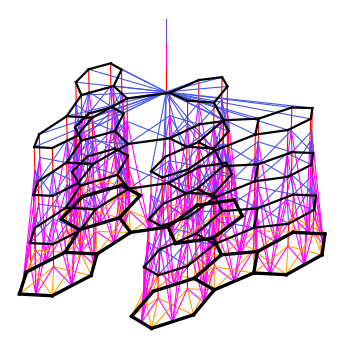
\includegraphics[width=0.4\textwidth]{figures/3d-nets/net1}}
\caption{A visualization of one of the convolutional nets constructed on a molecule.}
\label{placeholder}
\end{figure}

\begin{figure}
\centerline{
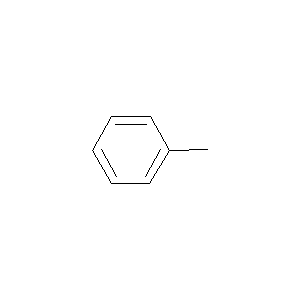
\includegraphics[width=0.2\textwidth]{figures/convnet-features/hidden-unit-0}
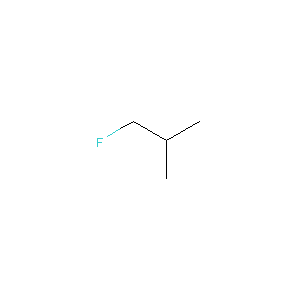
\includegraphics[width=0.2\textwidth]{figures/convnet-features/hidden-unit-1}}
\caption{The molecular fragments which most activate two of the features of the convolutional net.}
\label{placeholder}
\end{figure}


\section{Related work}

\paragraph{Fingerprints}

[Cite Morgan] and \cite{ECFP2010} developed extended circular fingerprints.
These fingerprints map identical molecules to the same set of fingerprints.
These same fingerprints have been pressed into service as a measure of similarity.

However, for a meaningful measure of similarity, 

\paragraph{Convolutional Neural Networks}

Convolutional neural networks have been used to model images, speech, and time series\cite{lecun1995convolutional}.
However, standard convolutional architectures use a fixed computational graph, making them difficult to apply to objects of varying size or structure, such as molecules.
More recently, \cite{KalchbrennerACL2014} developed a convolutional neural network architecture for modeling sentences of varying length and structure.

\paragraph{Recursive Neural Networks}

\cite{socher2011semi} and \cite{socher2011dynamic} use a pyramidal architecture for performing inference on variable-length sentences.

\paragraph{Neural nets for QSAR}

\cite{dahl2014multi} used standard deep neural networks, and didn't do any feature engineering.

\paragraph{Machine learning for identifying promising molecules}

\cite{Eckert2007225, bergeron2011modeling} provide reviews of the field.
\cite{tingley2014towards} used a variety of standard machine learning algorithms to predict the photovoltaic efficiency of organic molecules.

\paragraph{Neural Networks on Graphs}

\cite{graphnn2009} The Graph Neural Network Model

\cite{micheli2009neural} Neural network for graphs



\section{Experiments}

[How much is conceptual purity worth?  We can try using only topology, or include lots of hand-engineered features that we think will be useful.]

\subsection{Are Morgan fingerprints basically a hash function for molecules?}

We can answer this question by evaluating the performance of neural fingerprints generated by randomly initialized weights.


Predicting molecular weight:

Mean predictor
Performance (RMSE):
Train: 241.630442201
Test:  243.609627269

Fingerprints with linear weights
Performance (RMSE):
Train: 142.774743361
Test:  151.932246613

Random net with linear weights
Performance (RMSE):
Train: 144.492288513
Test:  150.182390847



\subsection{Datasets}

\subsection{Interpretability}
[Idea: Use nested dropout to allow a variable-sized descriptor.]
Explain that it's analogous to PCA for neural nets

[Wishlist: Include figures showing which fragments maximally activate different features - hopefully showing that they correspond to interpretable, familiar concepts]








%----------------------------------------------------------------------------------------
%	MATERIALS AND METHODS
%----------------------------------------------------------------------------------------

%% Optional Materials and Methods Section
%% The Materials and Methods section header will be added automatically.

\begin{materials}
\end{materials}





%----------------------------------------------------------------------------------------
%	APPENDICES (OPTIONAL)
%----------------------------------------------------------------------------------------

\appendix
An appendix without a title.

\appendix[Appendix title]
An appendix with a title.






%----------------------------------------------------------------------------------------
%	ACKNOWLEDGEMENTS
%----------------------------------------------------------------------------------------

\begin{acknowledgments}
This work was partially supported by a grant from the Spanish Ministry of Science and Technology.
\end{acknowledgments}






%----------------------------------------------------------------------------------------
%	BIBLIOGRAPHY
%----------------------------------------------------------------------------------------

%% PNAS does not support submission of supporting .tex files such as BibTeX.
%% Instead all references must be included in the article .tex document. 
%% If you currently use BibTeX, your bibliography is formed because the 
%% command \verb+\bibliography{}+ brings the <filename>.bbl file into your
%% .tex document. To conform to PNAS requirements, copy the reference listings
%% from your .bbl file and add them to the article .tex file, using the
%% bibliography environment described above.  

%%  Contact pnas@nas.edu if you need assistance with your
%%  bibliography.

% Sample bibliography item in PNAS format:
%% \bibitem{in-text reference} comma-separated author names up to 5,
%% for more than 5 authors use first author last name et al. (year published)
%% article title  {\it Journal Name} volume #: start page-end page.
%% ie,
% \bibitem{Neuhaus} Neuhaus J-M, Sitcher L, Meins F, Jr, Boller T (1991) 
% A short C-terminal sequence is necessary and sufficient for the
% targeting of chitinases to the plant vacuole. 
% {\it Proc Natl Acad Sci USA} 88:10362-10366.


%% Enter the largest bibliography number in the facing curly brackets
%% following \begin{thebibliography}
%\begin{thebibliography}
%\bibliography{references}
%\end{thebibliography}

\bibliographystyle{pnas2011}
\bibliography{references}

%----------------------------------------------------------------------------------------

\end{article}

%----------------------------------------------------------------------------------------
%	FIGURES AND TABLES
%----------------------------------------------------------------------------------------

%% Adding Figure and Table References
%% Be sure to add figures and tables after \end{article}
%% and before \end{document}

%% For figures, put the caption below the illustration.
%%
%% \begin{figure}
%% \caption{Almost Sharp Front}\label{afoto}
%% \end{figure}



%% For Tables, put caption above table
%%
%% Table caption should start with a capital letter, continue with lower case
%% and not have a period at the end
%% Using @{\vrule height ?? depth ?? width0pt} in the tabular preamble will
%% keep that much space between every line in the table.

%% \begin{table}
%% \caption{Repeat length of longer allele by age of onset class}
%% \begin{tabular}{@{\vrule height 10.5pt depth4pt  width0pt}lrcccc}
%% table text
%% \end{tabular}
%% \end{table}

\begin{table}[h]
\caption{Table caption}\label{sampletable}
\begin{tabular}{l l l}
\hline
\textbf{Treatments} & \textbf{Response 1} & \textbf{Response 2}\\
\hline
Treatment 1 & 0.0003262 & 0.562 \\
Treatment 2 & 0.0015681 & 0.910 \\
Treatment 3 & 0.0009271 & 0.296 \\
\hline
\end{tabular}
\end{table}


\begin{algorithm}
  \caption{Pseudocode of ECFP}
  \textbf{Input:} {molecule m, radius $r$, atom features $g$, hash function $h$}
  \begin{algorithmic}
    \For {each atom $a$ in molecule} 
	    \State $r_a \leftarrow g(a)$ \Comment {Represent each atom by given properties}
    \EndFor
    \For {$\ell = 1$ to $r$} \Comment {Repeat for as many iterations as the radius}
	    \For {each atom $a$ in molecule}
		    \State $v \leftarrow c[r_a, r_{n1} \dots r_{nN} ]$ \Comment {Concatenate representation of self and neighbours}	    
		    \State $r_a \leftarrow h(v)$ \Comment {Compute hash of concatenated representation}
	    \EndFor
    \EndFor
    \For {each feature $f$ in bitstrings}
	    \State $o_f \leftarrow \max[r_{1f} \dots r_{Mf}]$ \Comment {Combine duplicate features by a max or sum}
    \EndFor    
  \end{algorithmic}
\end{algorithm}

\begin{algorithm}
  \caption{Pseudocode of Neural Fingerprints}
  \textbf{Input:} {molecule m, radius $r$, learned atom vectors $g$, {\color{blue} learned smooth functions $f_1 \dots f_r$}}
  \begin{algorithmic}
    \For {each atom $a$ in molecule} 
	    \State $r_a \leftarrow g(a)$ \Comment {Represent each atom by a learned vector}
    \EndFor
    \For {$\ell = 1$ to $r$} \Comment {For R layers}
	    \For {each atom $a$ in molecule}
		    \State $v \leftarrow c[r_a, r_{n1} \dots r_{nN} ]$ \Comment {Concatenate representation of self and neighbours}	    
		    \State $r_a \leftarrow {\color{blue}f_{\ell}}(v)$ \Comment {Compute learned, smooth function of concatenated representation}
	    \EndFor  \Comment {Each layer's smooth function can be distinct}
    \EndFor
    \For {each feature $f$ in bitstrings}
	    \State $o_f \leftarrow \max[r_{1f} \dots r_{Mf}]$ \Comment {Combine duplicate features by a max or sum}
    \EndFor    
  \end{algorithmic}
\end{algorithm}

%% For two column figures and tables, use the following:

%% \begin{figure*}
%% \caption{Almost Sharp Front}\label{afoto}
%% \end{figure*}

%% \begin{table*}
%% \caption{Repeat length of longer allele by age of onset class}
%% \begin{tabular}{ccc}
%% table text
%% \end{tabular}
%% \end{table*}

%----------------------------------------------------------------------------------------

\end{document}